\documentclass[10pt]{beamer}

%\documentclass[10pt, handout]{beamer}
\setbeameroption{show notes}

%\documentclass[10pt, a4paper]{article}
%\usepackage{beamerarticle}




\mode<article>{
	
	\usepackage{hyperref}
	
}
\mode<presentation>{
	
	\usetheme{Antibes}
	\usefonttheme{professionalfonts} 
	\usefonttheme{serif} % default family is serif
	
	%\usecolortheme{spruce} %зеленая, плохой цвет в заголовках 
	%\usecolortheme{albatross} %синяя, пхоло виден черный цвет
	
}

\newcommand{\MP}[1]{\mode<presentation>{#1} }
\newcommand{\MA}[1]{\mode<article>{#1} }

\newcommand{\ABS}[1]{\left| #1 \right|}
%\newcommand{\ABS}[1]{\mid #1 \mid}

\newcommand{\HREF}[2]{{\color{blue}\underline{\href{#1}{#2}}}}

\setbeamertemplate{caption}[numbered]


%\usepackage[T2A]{fontenc}
%\usepackage[utf8]{inputenc}
%\usepackage[russian]{babel}
%\usepackage{amsmath} %математические формулы



\usepackage{ifthen}

\usepackage{tikz}
\usetikzlibrary{arrows.meta}
\usetikzlibrary{calc}
\usetikzlibrary{decorations}
\usetikzlibrary{decorations.pathreplacing}
\newcommand{\rememb}[1]{\tikz[remember picture,baseline=-0.5ex]{\draw node[inner sep=0pt, outer sep=0pt] (#1){\strut};}}



\usepackage{fp}
\usepackage{tikz-3dplot}
\usepackage{environ}
\usepackage{animate}





\usepackage{xcolor}
%\usepackage[left=20mm,right=20mm,top=20mm,bottom=20mm,a4paper]{geometry} %поля

\usepackage{amsmath} %математические формулы
%\usepackage{amsfonts} %математические шрифты


\usepackage[e]{esvect}  %Красивая стрелочка вектора
%\let\oldvv\vv
\newcommand{\VV}[1]{\vv{#1\mathstrut}}



\usepackage{graphicx} %работа с каритнками


%\usepackage{multimedia}
%\usepackage{movie15}

%Для XeLatex/+
\usepackage{polyglossia}
\setdefaultlanguage{russian}
\setotherlanguage{english}
%\setkeys{russian}{babelshorthands=true} 


\usepackage{fontspec}

\setmainfont{Times New Roman} [Script=Cyrillic, Mapping=tex-text,]
\setsansfont{Arial} [Script=Cyrillic, Mapping=tex-text,]
%\setmonofont{Courier New} [Script=Cyrillic, Mapping=tex-text,]
\newfontfamily{\cyrillicfonttt}{Courier New}


%\usepackage{unicode-math}
%\setmathfont{TeX Gyre Termes Math}

%\setmainfont{CMU Serif}[Script=Cyrillic, Mapping=tex-text,]
%\setsansfont{CMU Sans Serif}[Script=Cyrillic, Mapping=tex-text,]
%\setmonofont{CMU Typewriter Text}[Script=Cyrillic, Mapping=tex-text,]


%-----------------


%\usepackage{caption}
%\DeclareCaptionLabelSeparator{dot}{~---~}            %Разделитель номер рисунка
%\captionsetup[figure]{justification=centering,labelsep=dot, format=plain}                        %Подпись рис. центр
%\captionsetup[table]{justification=raggedleft,labelsep=dot, format=plain, singlelinecheck=false} %Подпись табл. слева
%\captionsetup[lstlisting]{justification=raggedleft,labelsep=dot, format=plain, singlelinecheck=false}                     %Подпись рис. центр

\usepackage{indentfirst} %отступ первой строки


\usepackage[svgnames]{xcolor}


\usepackage{hyperref}

%\usepackage{showframe}


%\usepackage{tikz}

%\usepackage[hidelinks]{hyperref}%ссылки внутри документа \ref


\setlength\abovecaptionskip{-2pt}
%\setlength\belowcaptionskip{-14pt}

\setbeamerfont{caption}{size=\scriptsize}


\def\sectionname{Раздел}
\def\subsectionname{Подраздел}


\newcommand{\TC}[3]
{
	
	
	\begin{columns}
		\begin{column}{#1\textwidth}
			#2
		\end{column}
		\begin{column}{\fpeval{1-#1}\textwidth}
			#3
		\end{column}
	\end{columns}
}

\newcommand{\TCT}[3]
{
	
	\begin{columns}[T]
		\begin{column}{#1\textwidth}
			#2
		\end{column}
		\begin{column}{\fpeval{1-#1}\textwidth}
			#3
		\end{column}
	\end{columns}
}


\newcommand{\FRAME}[2]{
	\begin{frame}
		\frametitle{#1}
		#2
	\end{frame}
}

\newcommand{\FIG}[3]
{
	\begin{figure}
		\centering
		\includegraphics[width=#3]{#1}
		\caption{#2}
	\end{figure}
}

\newcommand{\vect}[1]{\overrightarrow{#1}}


\usepackage{qrcode}

\newcommand{\LECADDR}{https://clck.ru/3D3Efj}


\usepackage{newfile}

\edef\LectionNumber{0}
\edef\LectionTheme{0}

\let\oldsection\section
\let\oldsubsection\subsection


\AtBeginDocument
{
	\newoutputstream{CONTENT}
	\openoutputfile{\LectionNumber .gvr}{CONTENT}
	
	\expandafter\addtostream{CONTENT}{\noindent\textbf{\Large Лекция \LectionNumber~---~\LectionTheme}\unexpanded{\setcounter{SEC}{0}}\par}
}

\renewcommand{\section}[1]{
	\oldsection{#1}
	\expandafter\addtostream{CONTENT}{\noindent\hspace{2ex}\unexpanded{\hbox{\large\stepcounter{SEC}\theSEC ~ #1}}\par}
}

\renewcommand{\subsection}[1]{
	\oldsubsection{#1}
	\expandafter\addtostream{CONTENT}{\noindent\hspace{6ex}\unexpanded{\stepcounter{SUB}\theSUB ~ #1}\par}
}


%\renewcommand{\section}[1]{\MMM{#1}}

%\edef\subsection#1
{
	%\noexpand\subsection{#1}
	%
}


\newfontfamily\dnifamily[Scale = 0.795]{DniFont.TTF}

\newcommand{\dni}[1]{%
	{\dnifamily%
		\ifthenelse{#1=0}{0}{}%
		\ifthenelse{#1=1}{1}{}%
		\ifthenelse{#1=2}{2}{}%
		\ifthenelse{#1=3}{3}{}%
		\ifthenelse{#1=4}{4}{}%
		\ifthenelse{#1=5}{5}{}%
		\ifthenelse{#1=6}{6}{}%
		\ifthenelse{#1=7}{7}{}%
		\ifthenelse{#1=8}{8}{}%
		\ifthenelse{#1=9}{9}{}%
		\ifthenelse{#1=10}{)}{}%
		\ifthenelse{#1=11}{!}{}%
		\ifthenelse{#1=12}{@}{}%
		\ifthenelse{#1=13}{\#}{}%
		\ifthenelse{#1=14}{\$}{}%
		\ifthenelse{#1=15}{\%}{}%
		\ifthenelse{#1=16}{\^{}}{}%
		\ifthenelse{#1=17}{\&}{}%
		\ifthenelse{#1=18}{*}{}%
		\ifthenelse{#1=19}{(}{}%
		\ifthenelse{#1=20}{[}{}%
		\ifthenelse{#1=21}{]}{}%
		\ifthenelse{#1=22}{\textbackslash{}}{}%
		\ifthenelse{#1=23}{\{}{}%
		\ifthenelse{#1=24}{\}}{}%
		\ifthenelse{#1=25}{|}{}}%
}%

\newcommand{\toDni}[1]{%	
	\ifthenelse{#1=0}{}{%
		 \ifthenelse{#1=25}{%
		 	\expandafter\dni{#1}}{%
		 	\expandafter\toDni{\fpeval{floor(#1/25)}}%
		 \expandafter\dni{\fpeval{(#1/25 - floor(#1/25))/0.04}}}}%
}%



\newcommand{\Strut}{{\Large\strut}}

\newcommand\scb[1]{\left( #1 \right)}

\newcommand{\LINK}[2]{%
	\qrcode[height=1cm]{#1}\  \HREF{#1}{\parbox{0.8\textwidth}{#2}} \\[0.5em]
}

\NewDocumentCommand{\lecdni}{}{\toDni{\LectionNumber}}
\author{Гаврилов Андрей Геннадьевич}
\newcommand{\regals}{кандидат технических наук, доцент}
\institute{Кафедра Информационных технологий и вычислительных систем \\МГТУ~<<СТАНКИН>>}
\lecture{История компьютерной графики}{kghistory}\subtitle{Компьютерная графика}


\makeatletter
\newcommand*{\overlaynumber}{\number\beamer@slideinframe}
\makeatother



\usepackage{cprotect}

\newcommand{\QRFRAME}{%
    \begin{frame}[plain, noframenumbering]    	
	
	\centering
	Трансляция презентации (во время очных лекций)    
	
	~
	
	{\Large \ttfamily  https://clck.ru/3D3Efj  }
	
	~
	
	\tikz\node[inner sep=0pt,rounded corners=5mm, clip]{\qrcode[height=0.45\textwidth]{\LECADDR}}; 
	
	~	
	{\small
	При просмотре презентации в PDF для отображения анимаций на слайдах необходимо использовать Acrobat Reader, KDE Okular, PDF-XChange, Foxit Reader, браузер Firefox. Для браузеров на движке Chrome (Edge, Яндекс, Opera,~\dots) необходимо использовать \HREF{https://chromewebstore.google.com/detail/pdf-viewer/oemmndcbldboiebfnladdacbdfmadadm?hl=ru&utm_source=ext_sidebar}{PDF.js} c опцией <<Enable active content (JavaScript) in PDFs>>. }
	
	\end{frame}%
}

\newcommand{\IG}[2][1]{\includegraphics[width=#1\textwidth]{#2}}



\graphicspath{{Images/}{Images/\jobname/}}

\date{\today}



\renewcommand{\LectionNumber}{9}
\renewcommand{\LectionTheme}{Закраска объектов и освещение}
\title{Лекция \lecdni \\ \LectionTheme}
\subtitle{Компьютерная графика}



%\usepackage{standalone}

\setbeamersize
{
	text margin left=0.5cm,
	text margin right=0.5cm
}

\usepackage{comment}


%	\transduration{2}
%   \transfade

 \begin{document}
 		 
	\makeatletter
\defbeamertemplate*{title page}{my theme}
{
	
	\hfill
	
	\begin{beamercolorbox}[wd=.9\paperwidth,center,]{title}%
		
	\end{beamercolorbox}%	
	
	\vbox to 1em {}
	
	\begin{beamercolorbox}[wd=.9\paperwidth,center,]{title}%
		\usebeamerfont{subtitle}%
		\hfill
		
		\insertsubtitle
		
		\usebeamerfont{title}%
		\inserttitle{} \\[0.5em]
		
		
		
	\end{beamercolorbox}%	
	\hfill\hfill
	
	\begin{beamercolorbox}[wd=.9\paperwidth,center,]{}%
		\usebeamerfont{author}%
		\hfill \\[0.5em]
		\insertauthor{} \\[0.5em]
		\regals
		    
		\vbox to 1em{}
		\usebeamerfont{institute}%
		\insertinstitute {}
		
		\vbox to 1em{}			
		{\; }\insertshortdate{}
		
	\end{beamercolorbox}%	
	\hfill\hfill
	
	\vbox to 5em{}
	
	
}
\defbeamertemplate*{footline}{my theme}{
	\leavevmode%
	\hbox{%
		\begin{beamercolorbox}[wd=.25\paperwidth,ht=3.25ex,dp=0ex,center,sep=1pt]{author in head/foot}%
			\usebeamerfont{author in head/foot}%
			\insertauthor 
			\beamer@ifempty{\insertshortinstitute}{}
		\end{beamercolorbox}%
		\begin{beamercolorbox}[wd=.65\paperwidth,ht=3.25ex,dp=0ex,center,sep=1pt]{title in head/foot}%
			\usebeamerfont{title in head/foot}\insertshortinstitute
		\end{beamercolorbox}%
		\begin{beamercolorbox}[wd=.1\paperwidth,ht=3.25ex,dp=0ex,center, sep=0.5pt]{date in head/foot}%
			\usebeamerfont{date in head/foot}
			\footnotesize \expandafter\toDni{\insertframenumber} / \expandafter\toDni{\inserttotalframenumber}
	\end{beamercolorbox}}%
}



\makeatother






%float page top aligment
\makeatletter
\setlength{\@fptop}{0pt}
\setlength{\@fpbot}{0pt plus 1fil}
\makeatother

\newcommand \abs[1] {\left| #1 \right|}

\everymath{\displaystyle}

    
    \QRFRAME	
	

	\frame{\maketitle}

	
	\begin{frame}{План лекции}
		\tableofcontents
	\end{frame}
	

	
	\begin{frame}{Red Dead Redemption 2 + shading mod}
		
		\centering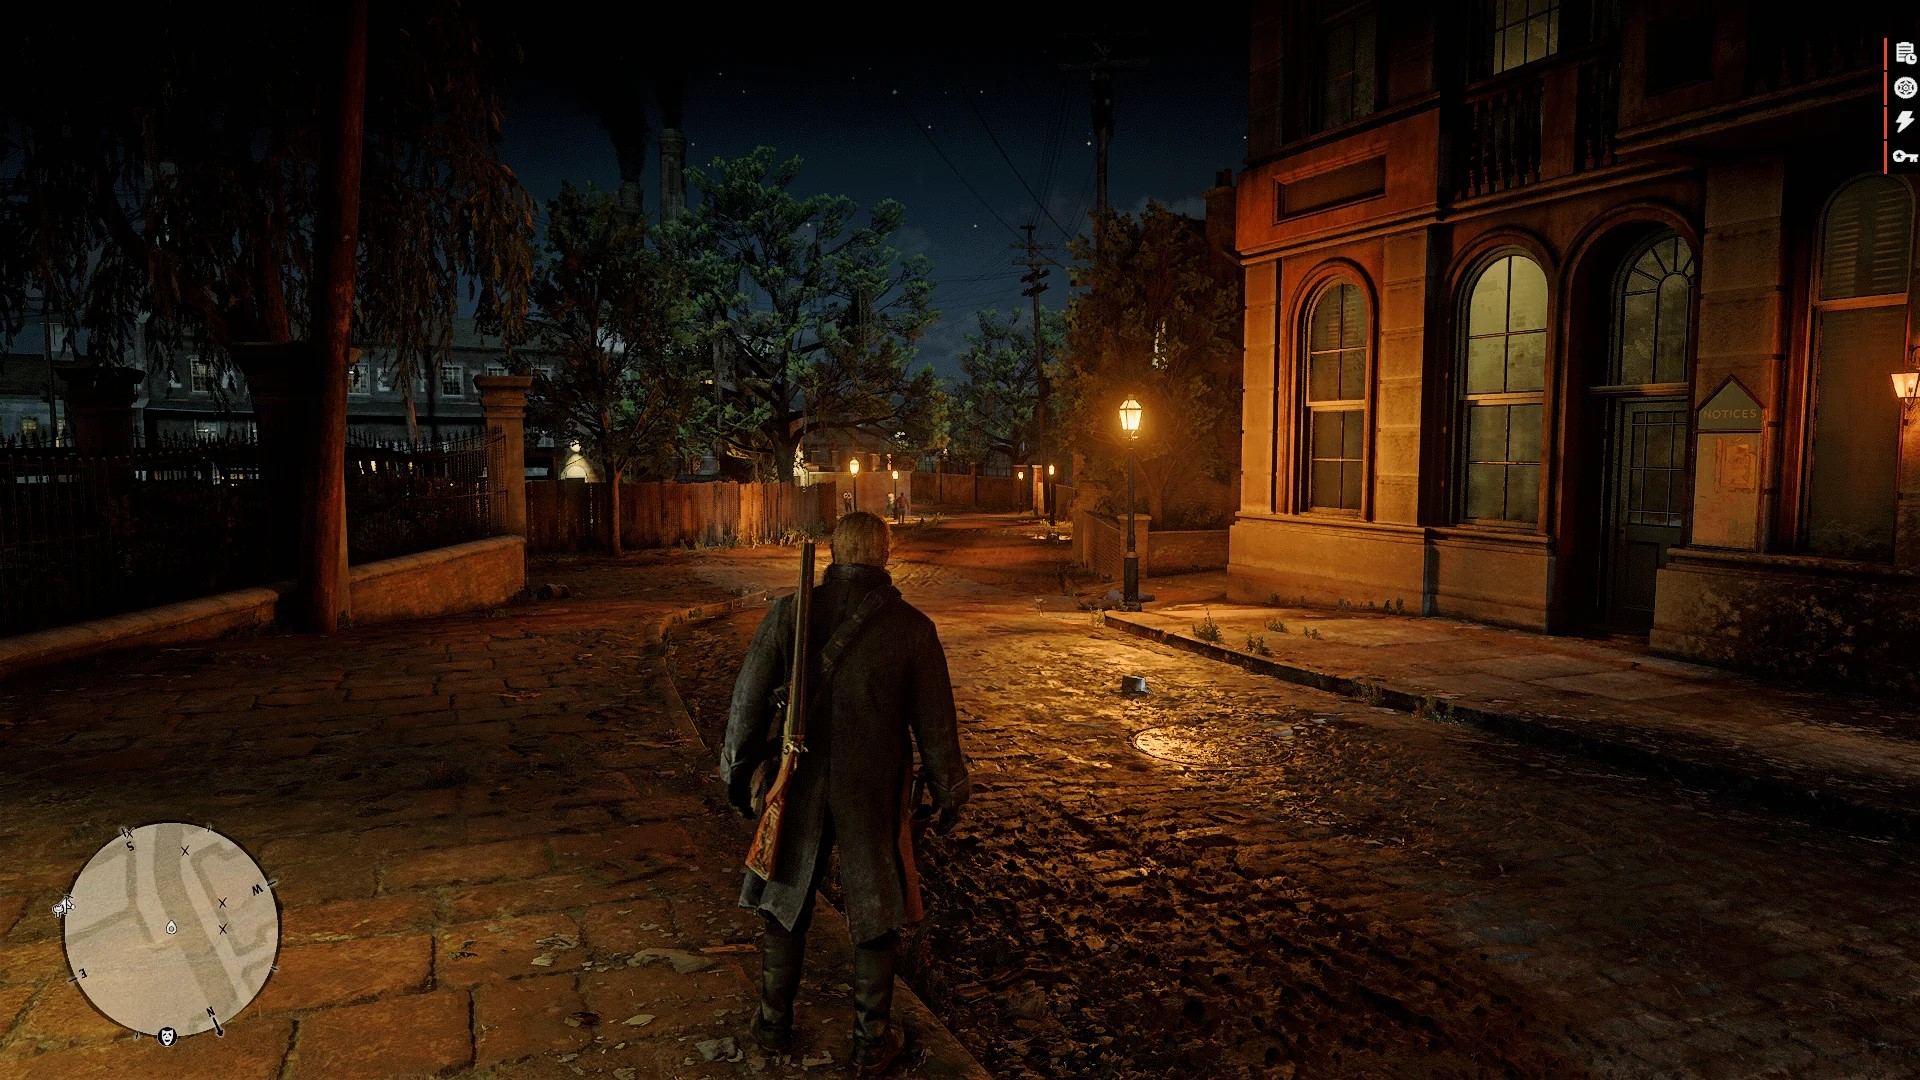
\includegraphics[width=0.95\textwidth]{rdr2}
		
	\end{frame}	
	
	
	\begin{comment}
		
	
	\begin{frame}{Обозначения}
		\TC{0.5}
		{
			\includegraphics[page=1]{light.pdf}
			
		}
		{
			$\vv l$ --- направление на источник света
			
			~
			
			$\vv v$ --- направление на наблюдателя (камеру)
			
			~
			
			$\vv n$ --- вектор нормали
			
			~
			
			$\vv r$ --- $v$ отражённый от $\vv n$, $\vv r = 2\vv n (\vv n \cdot \vv v) - \vv v$
			
			~
			
			$\vv h$ --- биссектор векторов $\vv v$ и $\vv l$, $\vv h =\dfrac{\VV v + \VV l}{\ABS{\VV v+ \VV l}}$
			
		}
	
			
	\end{frame}	
	
	\end{comment}
	
	\section{Модели освещения}
	
	\begin{frame}{Компоненты освещения}
		\centering
		$I=I_a+I_d+I_s$
		
		~
		
		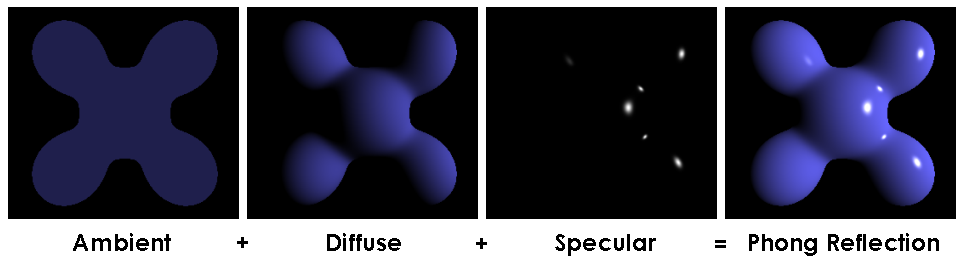
\includegraphics[width=0.8\textwidth]{components}
	\end{frame}
	
	\subsection{Модель Ламберта}
	
	\begin{frame}{Модель Ламберта}
		
			
		\TC{0.45}		
		{			
			\centering\includegraphics[page=2]{light.pdf}			
			
		}
		{
			 $I=\max\big(0,(\VV l \cdot \VV n)\big)$
			 
			 ~
			
			$\abs{\VV l}=\abs{\VV n}=1 \ \Rightarrow \ (\VV l \cdot \VV n) = \cos(\widehat{\VV l \cdot \VV n})$
			
			~
			
			\centering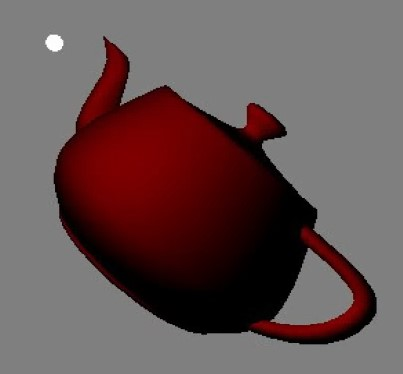
\includegraphics[width=0.7\textwidth]{lambert}
		}
		
	\end{frame}
\subsection{Wrap-around}
	\begin{frame}{Wrap-around}
		\centering $I=\dfrac{\max\big(0,(\VV l \cdot \VV n)\big)+f}{1+f}$
		
		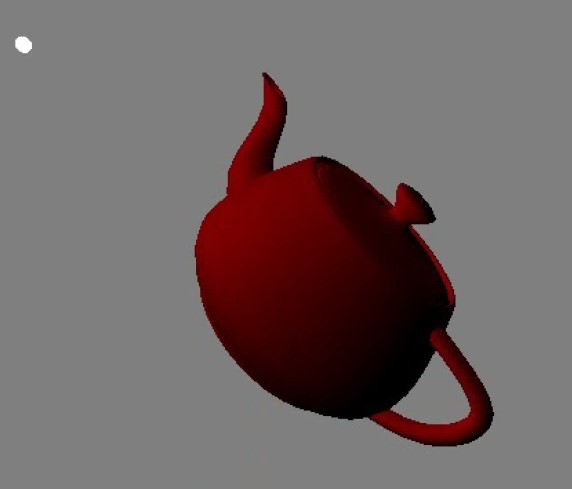
\includegraphics[width=0.4\textwidth]{warp.jpg}~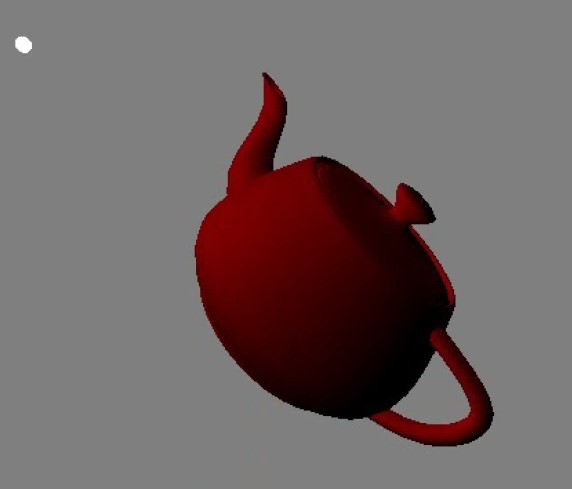
\includegraphics{warp.pdf}
	\end{frame}
 
 \begin{frame}{Модель Фонга (Phong lightning model)}
 	\TC{0.5}
 	{
 		\centering\includegraphics[page=3]{light.pdf}	
 	}
 	{
 		$\vv r=2\VV n(\VV l \cdot \VV n) - \VV l$
 		
 		~
 		
 		$I_d=\max\big(0,(\VV l \cdot \VV n)\big)$
 		
 		~
 		
 		$I_s=\max\big(0,(\vv v \cdot \vv r)^k \big)$
 		
 		~
 		
 		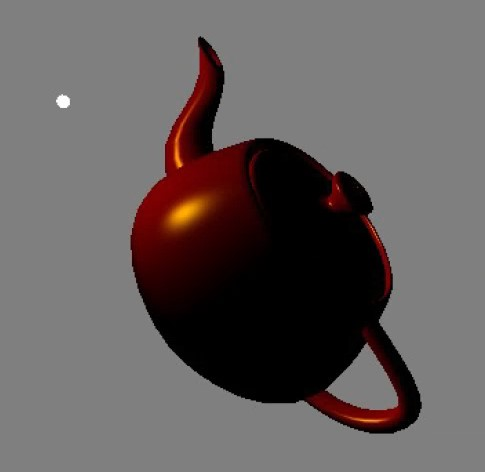
\includegraphics[width=0.7\textwidth]{phong.jpg}
 	}
 	

 	
 \end{frame}
 \subsection{Модель Фонга}
 
  \begin{frame}{Модель Фонга (Phong lightning model)}
 	\TC{0.35}
 	{
 		\centering\includegraphics[page=3]{light.pdf}	
 	}
 	{
 		
 		\quad\quad\quad\quad$I_s=\max\big(0,(\vv v \cdot \vv r)^k \big)$
 		
 		~
 		
 		~
 		
 		~
 		
 		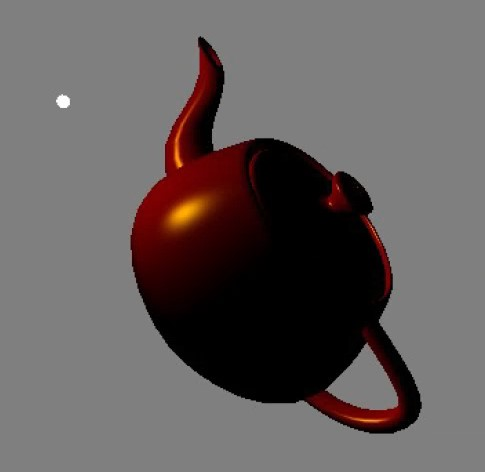
\includegraphics{phong.pdf}
 	}
 	\end{frame}
 	
 	\subsection{Модель Блинна}
 
 \begin{frame}{Модель Блинна  (Фонга - Блинна)}
 	
 	\TC{0.5}
 	{
 		\centering\includegraphics[page=4]{light.pdf}	
 	}
 	{
 		$\vv h=\dfrac{\VV l + \vv v}{\abs{\VV l + \VV v}}$ --- биссектор $\vv l$ и $\vv v$
 		
 		
 		~
 		
 		$I_s=\max\big(0,(\VV v \cdot \VV h)^k \big)$
 		
 		~
 		
 		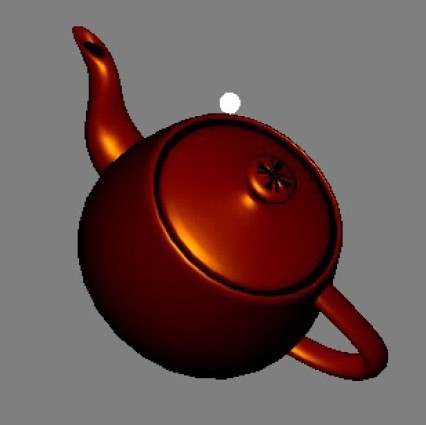
\includegraphics[width=0.7\textwidth]{blinn.jpg}
 	}
 	
 \end{frame}
 
 \subsection{Модель Варда}
 
 \begin{frame}{Модель Варда}
 	
 	\TC{0.5}
 	{
 		\centering\includegraphics[page=5]{light.pdf}
 		
 		
 	}
 	{
 		 		
 		$I_s=\exp\left(-k\dfrac{1-\left(\VV h\cdot \VV n\right)^2}{\left(\VV h\cdot \VV n\right)^2}\right)$
 		
 		
 		
 		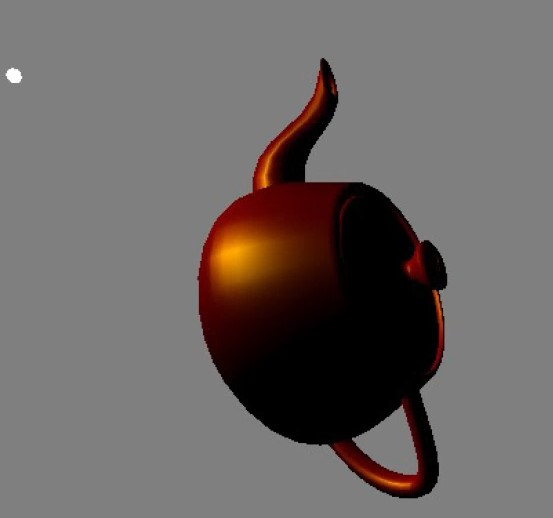
\includegraphics[width=0.7\textwidth]{ward.jpg}
 	

 	}
 	
 \end{frame}
 
  
 \begin{frame}{Модель Варда}
 	
 	\TC{0.4}
 	{
 		\centering\includegraphics[page=5]{light.pdf}
 		
 		
 	}
 	{
 		
 		\hspace{1cm}$I_s=\exp\left(-k\dfrac{1-\left(\VV h\cdot \VV n\right)^2}{\left(\VV h\cdot \VV n\right)^2}\right)$
 		
 		
 		
 		~
 		
 		~
 		
 		\moveleft  1cm \hbox{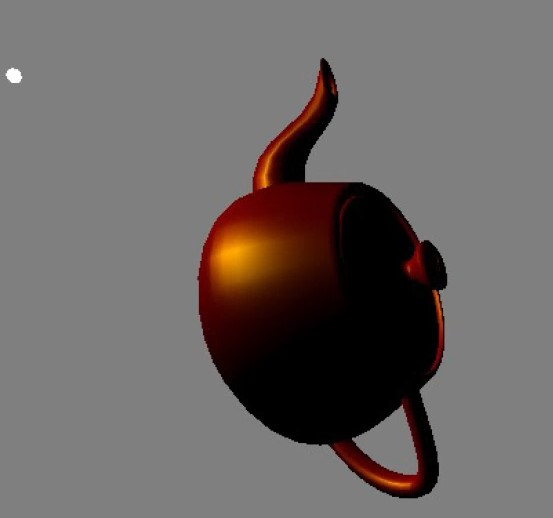
\includegraphics{ward.pdf}}
 		
 		
 	}
 	
 \end{frame}
 
 \subsection{Модель Орена - Наяра}
 \begin{frame}{Модель Орена - Наяра}
 	
 	 \small
 	 $L_r = L_1+L_2,$,
 	
 	$L_1 = \frac{\rho}{\pi} E_0 \cos \theta_i \left(C_1 + C_2 \cos(\phi_i-\phi_r) \tan\beta + C_3(1-|\cos(\phi_i-\phi_r)|)\tan\frac{\alpha+\beta}2\right)$,
 	
 	$L_2 = 0.17\frac{\rho^2}\pi E_0 \cos\theta_i\frac{\sigma^2}{\sigma^2+0.13}\left[1-\cos(\phi_i-\phi_r)\left(\frac{2\beta}\pi\right)^2\right]$,
 	
 	где
 	
 	$C_1 = 1-0.5\frac{\sigma^2}{\sigma^2+0.33}$,
 	
 	$C_2 = \begin{cases}
 		0.45\frac{\sigma^2}{\sigma^2+0.09}\sin\alpha & \text{если }\cos(\phi_i-\phi_r)\ge0,\\
 		0.45\frac{\sigma^2}{\sigma^2+0.09}\left(\sin\alpha-\left(\frac{2\beta}\pi\right)^3\right) & \text{иначе,}
 	\end{cases}$
 	
 	$C_3 = 0.125\frac{\sigma^2}{\sigma^2+0.09}\left(\frac{4\alpha\beta}{\pi^2}\right)^2$,
 	
 	$\alpha = \max(\theta_i, \theta_r)$,  	$\beta = \min(\theta_i, \theta_r)$
 	
 	$\rho$ --- альбедо поверхности, $\sigma$ --- шероховатость, $E_0$ --- освещение по Ламберту, 

 	
 \end{frame}
 
 \begin{frame}{Модель Орена - Наяра}
 	\TC{0.45}
 	{
 		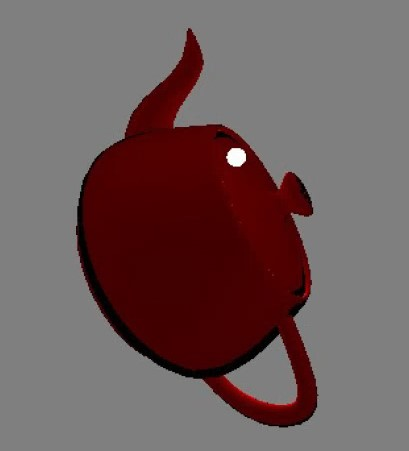
\includegraphics[width=0.99\textwidth]{oren3}
 	}
 	{
 		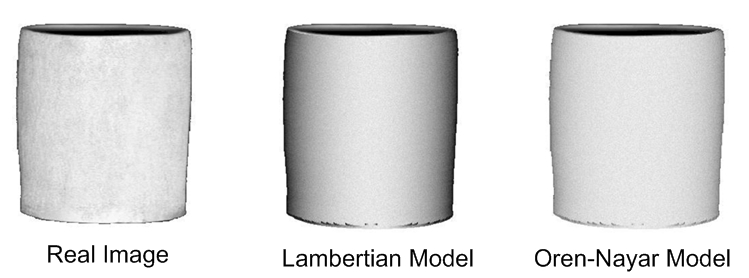
\includegraphics[width=0.99\textwidth]{oren1}
 		
 		~
 		
 		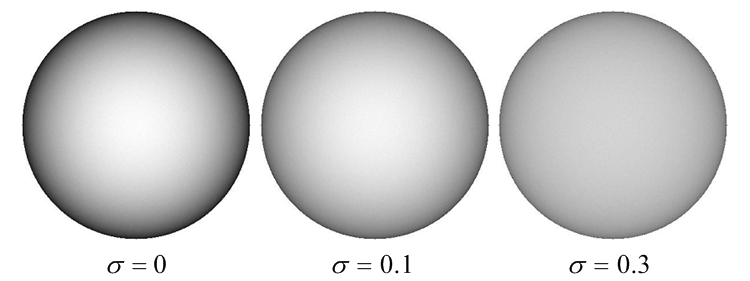
\includegraphics[width=0.99\textwidth]{oren2}
 	}
 	
 \end{frame}
 
  \subsection{Модель Кука-Торранса}
 
  \begin{frame}{Модель Кука-Торранса}


		\TC{0.5}
		{
			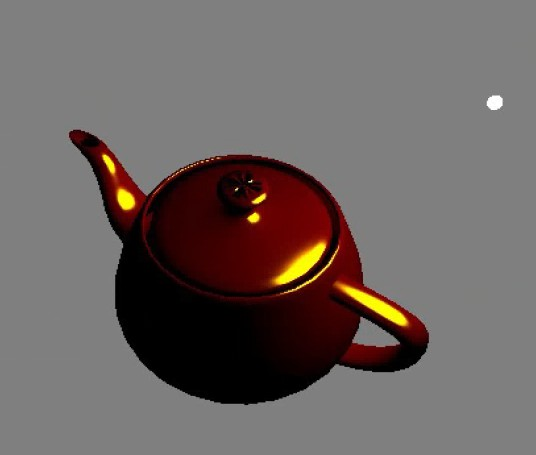
\includegraphics[width=\textwidth]{coock.jpg}	
		}
		{
			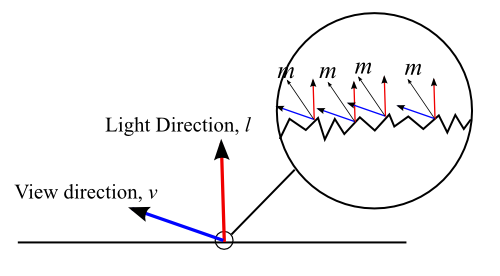
\includegraphics[width=\textwidth]{coock.png}	
		}
 	
 	
 \end{frame}
 
 \begin{frame}{Модель Кука-Торранса}
 	$I=I_d\left(sm_d+(1-s)I_s\right)$
 	
 	$I_s=\dfrac{DGF}{4\left(\VV n \cdot \VV l\right)\left(\VV n \cdot \VV v\right)}$
 	
 	$D$ --- функция распределения микрограней направленных на $h$.
 	Например $D=\frac{1}{\pi\alpha^2}\left(\VV h \cdot \VV n\right)^{\left(\tfrac{2}{\alpha^2} - 2\right)}$
 	
 	$G=\min\left(1,\dfrac{2\left(\VV h \cdot \VV n\right)\left(\VV n \cdot \VV v\right)}{\left(\VV v \cdot \VV h\right)}, \dfrac{2\left(\VV h \cdot \VV n \right)\left(\VV n \cdot \VV l\right)}{\left(\VV v \cdot \VV h\right)}\right)$
 	
 	$F$ --- эффект Френеля
 	
 	$F=F_0+\left(1-F_0\right)\left[1-\left(\VV v \cdot \VV h\right)\right], F_0=\frac{(n-1)^2}{(n+1)^2}$
 	
 	
 	
 	
 \end{frame}
 
 \section{Модели затенения}
 
 \subsection{Однотонная закраска}
 
 \begin{frame}{Однотонная закраска}
 	\TC{0.5}
 	{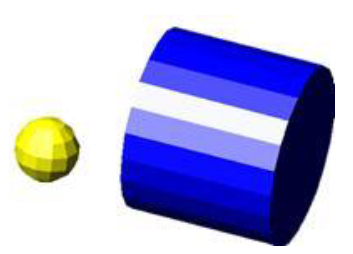
\includegraphics[width=\textwidth]{tone.png}
 	}{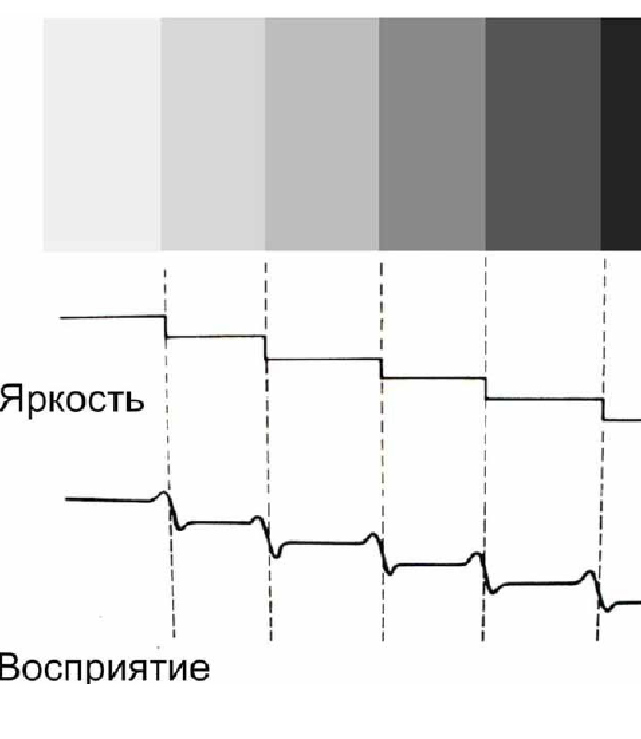
\includegraphics[width=\textwidth]{mach.png}
 	}
 \end{frame}
 
  \subsection{Закраска по Гуро}
  

  
  \begin{frame}{Закраска по Гуро}
  	\begin{tikzpicture}[font=\small]
  		\usetikzlibrary{calc}
  		\coordinate (A) at (0,0);
  		\coordinate (B) at (6,1);
  		\coordinate (C) at (2,4);
  		
  		\draw[thick] (A) -- (B) -- (C) -- cycle;
  		
  		\draw[-Latex] (A) -- +(90:1); 
  		\draw[-Latex] (B) -- +(60:1); 
  		\draw[-Latex] (C) -- +(120:1); 
  		
  		\coordinate (F1) at (-1, 2);
  		\coordinate (F2) at (6, 2);
  		
  		\coordinate (X1) at (intersection of A--C and F1--F2);
  		\coordinate (X2) at (intersection of B--C and F1--F2);
  		\coordinate (X) at ($(X1)!0.5!(X2)$);
  		
  		\draw (A) node [left] {$I_A$};
  		\draw (B) node [right] {$I_B$};
  		\draw (C) node [above right] {$I_C$};
  		
  		\fill (X1) circle (1.5pt) (X2) circle (1.5pt) (X) circle (1.5pt);  		
  		\draw (X1) node [above left, align=right] {$I_{X_1}=\mathrm{lerp}\left(I_A, I_B,\frac{AX_1}{AC}\right)$\\$X_1$};
  		\draw (X2) node [above right,align=left] {$I_{X_2}=\mathrm{lerp}\left(I_C, I_B, \frac{BX_2}{BC}\right)$\\$X_2$};
  		
  		\draw (X) node [below, align=center]{$X$\\$I_X=\mathrm{lerp}\left(I_{X_1},I_{X_2},\frac{X_1X}{X_1X_2}\right)$}; 
  		
  		\draw[thin] (F1) -- (F2);
  	\end{tikzpicture}
  \end{frame}
  
     \begin{frame}{Закраска по Гуро}
  	\TC{0.5}{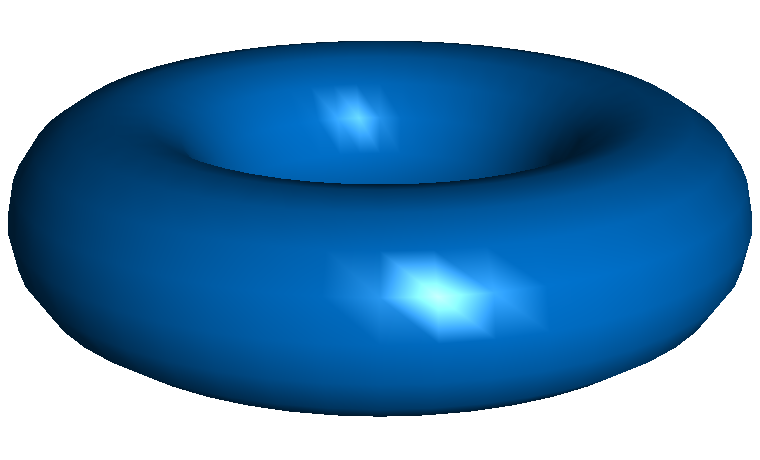
\includegraphics[width=\textwidth]{guro}}{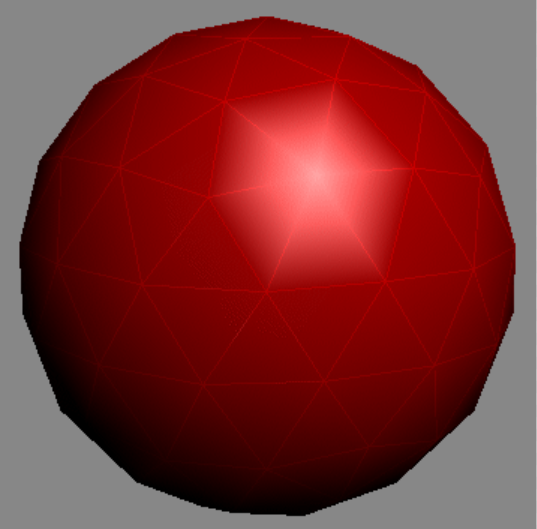
\includegraphics[width=\textwidth]{guro1}}
  \end{frame}
  
   \subsection{Закраска по Фонгу}
   
    \begin{frame} {Закраска по Фонгу}
  		\begin{tikzpicture}[font=\footnotesize]
  			\usetikzlibrary{calc}
  			\coordinate (A) at (0,0);
  			\coordinate (B) at (6,1);
  			\coordinate (C) at (2,4);
  			
  			\draw[thick] (A) -- (B) -- (C) -- cycle;
  			
  			\draw[-Latex] (A) -- +(90:1); 
  			\draw[-Latex] (B) -- +(60:1); 
  			\draw[-Latex] (C) -- +(120:1); 
  			  			
  			\coordinate (F1) at (-1, 2);
  			\coordinate (F2) at (6, 2);
  			
  			\coordinate (X1) at (intersection of A--C and F1--F2);
  			\coordinate (X2) at (intersection of B--C and F1--F2);
  			\coordinate (X) at ($(X1)!0.5!(X2)$);  			
  			
  			\foreach \t in {0.1,0.2,...,0.9}{
  				\coordinate (x1) at ($(A)!\t!(C)$);
  				\draw[-Latex, black!30] (x1) -- +($(90:1)!\t!(120:1)$);  
  				
  				\coordinate (x2) at ($(B)!\t!(C)$);
  				\draw[-Latex, black!30] (x2) -- +($(60:1)!\t!(120:1)$);  	
  				
  				\coordinate (x3) at ($(X1)!\t!(X2)$);
  				\draw[-Latex, black!30] (x3) -- +($(100:1)!\t!(80:1)$);  		
  			}
  			
  			\coordinate (x4) at ($(X1)!0.5!(X2)$);
  			\draw[-Latex] (x4) -- +($(100:1)!0.5!(80:1)$);  
  			
  			\draw (A) node [left] {$\vv N\!_A$};
  			\draw (B) node [right] {$\vv N\!_B$};
  			\draw (C) node [above right] {$\vv N\!_C$};
  			
  			\fill (X1) circle (1.5pt) (X2) circle (1.5pt) (X) circle (1.5pt);  		
  			\draw (X1) node [above left, align=right] {$\vv N\!_{X_1}=\mathrm{lerp}\left(\vv N\!_A, \vv N\!_B,\frac{AX_1}{AC}\right)$\\$X_1$};
  			\draw (X2) node [above right,align=left] {$\vv N\!_{X_2}=\mathrm{lerp}\left(\vv N\!_C, \vv N\!_B, \frac{BX_2}{BC}\right)$\\$X_2$};
  			
  			\draw (X) node [below, align=center, font=\footnotesize]{$X$\\$\vv N\!_X=\mathrm{lerp}\left(\vv N\!_{X_1},\vv N\!_{X_2},\frac{X\!_1X}{X\!_1X_2}\right)$}; 
  			
  			\draw[thin] (F1) -- (F2);
  		\end{tikzpicture}   	
   \end{frame}
   
   \begin{frame}{Закраска по Фонгу}
   	\centering
   	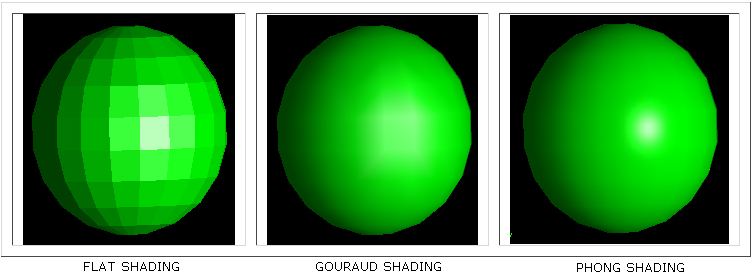
\includegraphics[width=0.8\textwidth]{shadingoptions.png}
   	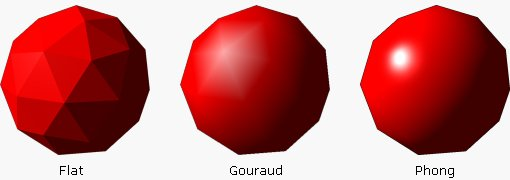
\includegraphics[width=0.8\textwidth]{fyAFK.jpg}
   	
   \end{frame}
 
\begin{comment}
	
\end{comment}
 

\end{document}